\section{Surface Wave Solutions}

A sample solution to our problem is shown in figure~\ref{f:FEM solution}. Note the domain includes a cusp.
% FIXME Give reference to cusp description in \ref{s:unperturbed structure}
Normally, producing a solution for a domain with a cusp would require special consideration. For the solution shown, domain triangulation was performed manually near the cusp and quadrature points were altered as well. Such an approach is not rigorous. Nonetheless, the solution produced near the cusp does not appear to display any singularities and this is promising since it suggests that the solution near the cusp does not exhibit any singularities.

\begin{figure}
\begin{center}
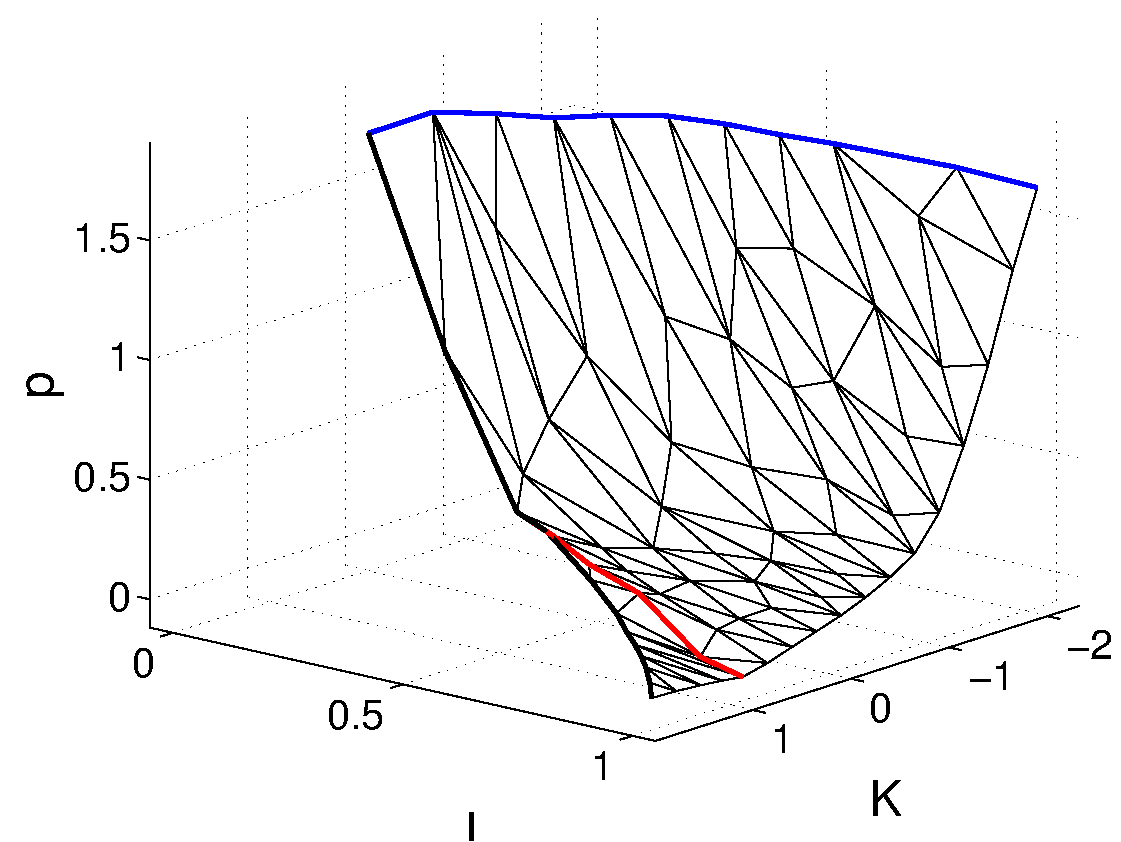
\includegraphics[width=\textwidth*7/8]{figures/db3_surf}
\caption{Probability density solution. Parameters are as the same as those for figure~\ref{f:drift diffusion figures}}
\label{f:FEM solution}
\end{center}
\end{figure}

With regards to physical significance of the solution, the main point to note is that the probability density function (PDF) is highest along the edge $K_{2I}$. This feature of the solution remains present when the aspect ratio of the cylindrical basin is varied from $d/a = 1$, as in Figure \ref{f:FEM solution} down to 0.3 (solution not illustrated.) In the X-Y phase plane, the edge $K_{2I}$ is situated outside the homoclinic orbit and our results suggests the wave motions most likely to be observed would be those corresponding to circular motion where for a given value of $I$, $K$ is near its maximum.

Similarly to our analysis, in \citet{miles84:_reson}, a system of two surface-gravity wave modes in a cylindrical basin subjected to horizontal excitation is studied. Unlike our problem, the two wave modes are set to be in exact resonance with one another, and a detuning parameter is introduced to represent the frequency difference between the natural wave frequency and the forcing frequency. A significant conclusion reached in that study is that for cylindrical basins with an aspect ratio between 0.3 and 0.5, limit cycles and chaotic motion are not possible, making the wave dynamics observed in that interval of aspect ratios qualitatively different from the dynamics seen outside that interval. In our case, with stochastic excitation, the probability densities obtained inside and outside the interval do not exhibit any qualitative differences; in both cases, the probability density is highest near the edge $K_{2I}$.
